\providecommand{\main}{..}
\documentclass[\main/ApuntesPL.tex]{subfiles}

% !TEX root = ../ApuntesPL.tex

\begin{document}
  \begin{tikzpicture}
    \node[rectangle, draw = black, align = center, rectangle split, rectangle split horizontal, rectangle split parts = 2] (cl1) {};
    \node[rectangle, draw = black, right = .2 of cl1, align = center, rectangle split, rectangle split horizontal, rectangle split parts = 2] (cl2) {};
    \node[rectangle, draw = black, right = .2 of cl2, align = center, rectangle split, rectangle split horizontal, rectangle split parts = 2] (cl3) {};

    \node[unit, right = of cl3, align = center] (ansi) {Analizador\\sintáctico};
    \node[err, below=of ansi] (err) {error};

    \node[rectangle, right=2of ansi, label={Árbol incontextual}] (t1) {$e_0$};
    \node[rectangle, below left =.5 of t1] (t2) {$e_1$};
    \node[rectangle, below right =.5 of t1] (t3) {$e_2$};
    \node[rectangle, below left =.5 of t3] (t4) {$e_3$};
    \node[rectangle, below right =.5 of t3] (t5) {$e_4$};
    \node[rectangle, below left =.5 of t4] (t6) {$e_5$};
    \node[rectangle, below right =.5 of t4] (t7) {$e_6$};
    \node[rectangle, below left =.5 of t7] (t8) {$e_7$};
    \node[rectangle, below right =.5 of t7] (t9) {$e_8$};

    \draw[myarrow] (cl3.east) -- ++(0,0) -> (ansi.west);
    \draw[myarrow] (ansi.south) -- ++(0,0) -> (err.north);
    \draw[myarrow] (ansi.east) -- ++(0,0) -> (t1.west);

    \path[thick]
      (t1.south)  edge (t2)
                  edge (t3)
      (t3.south)  edge (t4)
                  edge (t5)
      (t4.south)  edge (t6)
                  edge (t7)
      (t7.south)  edge (t8)
                  edge (t9);
  \end{tikzpicture}

  \bigskip
  \par
  Hipótesis: Las cadenas de clases léxicas generadas por el analizador léxico forman un lenguaje incontextual.

  \section{Recordatorio}
    \subsection{Gramática}
      Sea una GI (Gramática Incontextual), GI(N,T,P,S):
      \begin{itemize}
        \item N $\equiv$ alfabeto de no terminales $\Rightarrow$ clases sintácticas.
        \item T $\equiv$ alfabeto de terminales $\Rightarrow$ clases léxicas.
        \item P $\equiv$ conjunto de reglas de la forma A $\rightarrow$ $\alpha$, donde A $\in$ N y $\alpha$ $\in$ (NUT)$\ast$.
        \item S $\in$ N y es el símbolo inicial.
      \end{itemize}

      \bigskip
      \par
      Sea G $\equiv$ (N,T,P,S) $\rightarrow$ G denota un lenguaje L(G)
      \begin{itemize}
        \item Relación de derivación $\Rightarrow_G$ (0 $\Rightarrow$ si G se sobreentiende) $\Rightarrow$ $\subseteq$ (NUT)$\ast$ x (NUT)$\ast$\\
              \hspace{5mm}$\alpha$A$\beta$ $\wedge$ A $\rightarrow \gamma \in$ P entonces $\alpha$A$\beta \Rightarrow \alpha \gamma$B
        \item Se considera $\Rightarrow_\ast$ aplicar cero o más veces $\Rightarrow$.
      \end{itemize}

      \par
      L(G) = \{w $\in$ T$\ast$ $\mid$ S $\Rightarrow_\ast$ w\}

      \bigskip
      \par
      \textbf{e.g.} Número binario\\
      \hspace{5mm}N = \{N,B\}\\
      \hspace{5mm}T = \{0,1\}\\
      \hspace{5mm}P = {\color{blue}N} $\rightarrow$ B\\
      \hspace{13mm}{\color{blue}N} $\rightarrow$ NB\\
      \hspace{13mm}{\color{blue}B} $\rightarrow$ {\color{red}0}\\
      \hspace{13mm}{\color{blue}B} $\rightarrow$ {\color{red}1}\\
      \hspace{5mm}S = N\\
      \vspace{2mm}
      \hspace{5mm}Esto sería equivalente a dar tan solo las reglas(P), donde:
      \begin{itemize}
        \item El símbolo {\color{blue}azul} de la primera regla es el símbolo inicial(S).
        \item El conjunto de símbolos {\color{blue}azules} son los no terminales(N).
        \item El conjunto de símbolos {\color{red}rojos} son los terminales(T).
      \end{itemize}

      \bigskip
      \par
      La derivación se denomina \textit{mas a la izquierda} si siempre se reescribe el no terminal que está mas a la izquierda, equivalente para \textit{mas a la derecha}.\\
      \vspace{3mm}
      \hspace{5mm}\textbf{Derivación}\\
      \hspace{10mm}{\color{red}N} $\Rightarrow$ {\color{red}N}B $\Rightarrow$ N{\color{red}B}B $\Rightarrow$ {\color{red}N}1B $\Rightarrow$ B1{\color{red}B} $\Rightarrow$ {\color{red}B}10 $\Rightarrow$ 010\\
      \vspace{3mm}
      \hspace{5mm}\textbf{Derivación mas a la izquierda}\\
      \hspace{10mm}{\color{red}N} $\Rightarrow$ {\color{red}N}B $\Rightarrow$ {\color{red}N}BB $\Rightarrow$ {\color{red}B}BB $\Rightarrow$ 0{\color{red}B}B $\Rightarrow$ 01{\color{red}B} $\Rightarrow$ 010\\
      \vspace{3mm}
      \hspace{5mm}\textbf{Derivación mas a la derecha}\\
      \hspace{10mm}{\color{red}N} $\Rightarrow$ N{\color{red}B} $\Rightarrow$ {\color{red}N}0 $\Rightarrow$ N{\color{red}B}0 $\Rightarrow$ {\color{red}N}10 $\Rightarrow$ {\color{red}B}10 $\Rightarrow$ 010

    \subsection{Árbol de análisis sintáctico}
      \par
      La idea es obtener una representación única para cada sentencia.

      \bigskip
      \par
      \textbf{Árboles}
      \begin{itemize}
        \item La raíz está etiquetada con el símbolo inicial.
        \item Están ordenados, hay un órden en los hijos de los nodos (primer hijo, segundo hijo...).
        \item Los nodos internos están etiquetados por no terminales.
        \item Los nodos hoja están etiquetados por terminales o por $\epsilon$.
        \item Si un nodo está etiquetado por A y sus hijos por $\alpha$ entonces A $\rightarrow \alpha \in$ P.
      \end{itemize}

      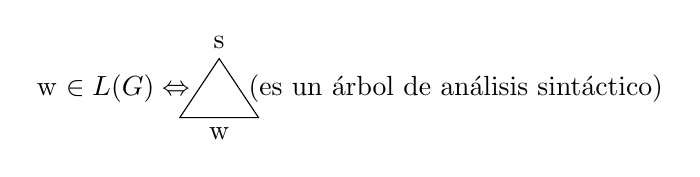
\begin{tikzpicture}
        \draw (0,0) node{}
          -- node[below]{w} (1,0) node{}
          -- node[right]{(es un árbol de análisis sintáctico)} (.5,.75) node[anchor=south]{s}
          -- node[left]{w $\in L(G) \Leftrightarrow$} cycle;
      \end{tikzpicture}

      \par
      \textbf{e.g.}\\
      \begin{center}
        \begin{minipage}{.2\textwidth}
          N $\rightarrow$ B\\
          N $\rightarrow$ NB\\
          B $\rightarrow$ 0\\
          B $\rightarrow$ 1
        \end{minipage}%
        \begin{minipage}{.3\textwidth}
          \begin{tikzpicture}
            \node[rectangle] (t1) {N};
            \node[rectangle, below left =.5 of t1] (t2) {N};
            \node[rectangle, below right =.5 of t1] (t3) {B};
            \node[rectangle, below left =.5 of t2] (t4) {N};
            \node[rectangle, below right =.5 of t2] (t5) {B};
            \node[rectangle, below =.5 of t3] (t6) {0};
            \node[rectangle, below =.5 of t4] (t7) {B};
            \node[rectangle, below =.5 of t5] (t8) {1};
            \node[rectangle, below =.5 of t7] (t9) {0};

            \path[thick]
              (t1.south) edge (t2)
                          edge (t3)
              (t2.south) edge (t4)
                          edge (t5)
              (t3.south) edge (t6)
              (t4.south) edge (t7)
              (t5.south) edge (t8)
              (t7.south) edge (t9);
          \end{tikzpicture}
        \end{minipage}%
        \begin{minipage}{.4\textwidth}
          \raggedright
          Cada nodo es equivalente a un array en el que se referencian sus hijos en orden.
        \end{minipage}
      \end{center}

  \section{Especificación sintáctica}
    \subsection{Determinar las clases sintácticas}
      \par
      ¿Cómo? A partir de la especificación informal.

      \bigskip
      \par
      De arriba a abajo:
      \begin{itemize}
        \item Identificar las clases complejas.
        \item Descomponerlas en clases más simples hasta llegar a las clases léxicas.
      \end{itemize}

      \bigskip
      \par
      Descomposición $\rightarrow$ Las clases resultantes deben estar al mismo nivel, el más alto posible.

      \bigskip
      \par
      \textbf{e.g.} L que describe libros
      \begin{center}
        \begin{minipage}{.4 \textwidth}
          \hspace*{5mm}Titulo [...]\\
          \hspace*{5mm}Autores [Autor]...[Autor]\\
          \hspace*{5mm}Capitulo [...][...]\\
          \hspace*{5mm}...\\
          \hspace*{5mm}Capitulo [...][...]
        \end{minipage}%
        \begin{minipage}{.5 \textwidth}
          \begin{tikzpicture}
            \node[rectangle] (lib) {Libro};
            \node[rectangle, below left =.8 of lib] (cab) {Cabecera};
            \node[rectangle, below right =.8 of lib] (cuer) {Cuerpo};
            \node[rectangle, below left =.5 of cab] (tit) {Titulo};
            \node[rectangle, below right =.5 of cab] (auts) {Autores};
            \node[rectangle, below =.5 of cuer] (cap) {Capitulo};
            \node[rectangle, below =.5 of auts] (aut) {Autor};
            \node[rectangle, below=.5 of cap] (tcap) {TituloCap};
            \node[rectangle, right=.5 of tcap] (ccap) {ContenidoCap};

            \path[thick]
              (lib.south) edge (cab)
                          edge (cuer)
              (cab.south) edge (tit)
                          edge (auts)
              (cuer.south) edge (cap)
              (auts.south) edge (aut)
              (cap.south) edge (tcap)
                          edge (ccap);
          \end{tikzpicture}
          \captionof{figure}{Árbol informal.}
        \end{minipage}
        \begin{minipage}{.4 \textwidth}
          \hspace*{5mm}Clases léxicas\\
          \hspace*{10mm}Autores\\
          \hspace*{10mm}Capitulo\\
          \hspace*{10mm}CAP\\
          \hspace*{10mm}CCIE\\
          \hspace*{10mm}Texto
        \end{minipage}%
        \begin{minipage}{.5 \textwidth}
          \vspace{10mm}
          \begin{tikzpicture}
            \node[rectangle, draw=black] (lib) {Libro};
            \node[rectangle, draw=black, below left =.8 of lib] (cab) {Cabecera};
            \node[rectangle, draw=black, below right =.8 of lib] (cuer) {Cuerpo};
            \node[rectangle, draw=black, below left =.6 and .5 of cab] (tit) {Title};
            \node[rectangle, draw=black, below right =.6 and .5 of cab] (auts) {Authors};
            \node[rectangle, draw=black, below =.5 of cuer] (cap) {Chapter};
            \node[rectangle, draw=black, below=.5 of cap] (tcap) {CTitle};
            \node[rectangle, draw=black, right=.5 of tcap] (ccap) {CContent};
            \node[rectangle, draw=black, below left=1.2 and 0 of tcap] (blo) {Bloque};
            \node[rectangle, draw=black, below =.5of blo] (tex) {Texto};

            \path[thick, ->]
              (lib.south) edge (cab)
                          edge (cuer)
              (cab.south) edge (tit)
                          edge (auts)
              (cuer.south) edge (cap)
              (tit.south) edge (blo)
              (auts.south) edge node[right, very near start] {+} (blo)
              (cap.south) edge (tcap)
                          edge (ccap)
              (tcap.south) edge (blo)
              (ccap.south) edge (blo)
              (blo.south) edge node[right] {$\ast$} (tex);
          \end{tikzpicture}
          \captionof{figure}{Árbol formal.}
        \end{minipage}
      \end{center}

    \subsection{Patrones para secuencias}
      \begin{itemize}
        \item Secuencia de 1 o más $I_s$, separados por $\Box$.\\
            \hspace{3mm}\textbf{e.g.} I $\mid$ I $\Box$ I $\mid$ I $\Box$ I $\Box$ I...\\
            \vspace{2mm}
            \hspace{3mm}LI $\rightarrow$ I\\
            \hspace{3mm}LI $\rightarrow$ LI $\Box$ I\\
            \vspace{2mm}
            \hspace{3mm}\textbf{e.g.}\\
            \hspace{3mm}NUM $\rightarrow$ B\\
            \hspace{3mm}NUM $\rightarrow$ NUM , B
        \item Secuencia de 0 o más $I_s$, separados por $\Box$.\\
            \hspace{3mm}S $\rightarrow$ $\varepsilon$\\
            \hspace{3mm}S $\rightarrow$ LI\\
            \hspace{3mm}LI $\rightarrow$ I\\
            \hspace{3mm}LI $\rightarrow$ LI $\Box$ I\\
            \vspace{2mm}
            \hspace{3mm}\textbf{e.g.} Declaraciones\\
            \hspace{3mm}Decs $\rightarrow$ $\varepsilon$\\
            \hspace{3mm}Decs $\rightarrow$ LDEC\\
            \hspace{3mm}LDEC $\rightarrow$ Dec\\
            \hspace{3mm}LDEC $\rightarrow$ LDEC ; Dec
      \end{itemize}

      \par
      Como caso particular de los patrones anteriores tenemos aquellos en que $\Box$ es
      $\varepsilon$, no están separados por nada.
      \begin{itemize}
        \item Secuencia de 1 o más $I_s$.\\
            \hspace{3mm}LI $\rightarrow$ I\\
            \hspace{3mm}LI $\rightarrow$ LI I
        \item Secuencia de 0 o más $I_s$.\\
            \hspace{3mm}S $\rightarrow$ $\varepsilon$\\
            \hspace{3mm}S $\rightarrow$ LI\\
            \hspace{3mm}LI $\rightarrow$ I\\
            \hspace{3mm}LI $\rightarrow$ LI I
      \end{itemize}

      \par
      También es posible usar un terminador en lugar de un separador para cada item.\\
      \hspace{3mm}\textbf{e.g.} \underline{I $\Box$} \underline{I $\Box$} \underline{I $\Box$}...
        donde I $\Box$ es un item.\\
      \begin{itemize}
        \item Secuencia de 1 o más $I_s$ terminados en $\Box$.\\
            \hspace{3mm}LI $\rightarrow$ BI\\
            \hspace{3mm}LI $\rightarrow$ LI BI\\
            \hspace{3mm}BI $\rightarrow$ I $\Box$\\
        \item Secuencia de 0 o más $I_s$ terminados en $\Box$.\\
            \hspace{3mm}S $\rightarrow$ $\varepsilon$\\
            \hspace{3mm}S $\rightarrow$ LI\\
            \hspace{3mm}LI $\rightarrow$ BI\\
            \hspace{3mm}LI $\rightarrow$ LI BI\\
            \hspace{3mm}BI $\rightarrow$ I $\Box$\\
      \end{itemize}

      \par
      \textbf{e.g.} Libro\\
      \begin{center}
        \begin{minipage}{.5\textwidth}
          \hspace*{5mm}Libro $\rightarrow$ Cabecera Cuerpo\\
          \hspace*{5mm}Cabecera $\rightarrow$ Title Authors\\
          \hspace*{5mm}Title $\rightarrow$ \underline{Titulo} Bloque\\
          \hspace*{5mm}Authors $\rightarrow$ \underline{Autores} LBloques\\
          \hspace*{5mm}LBloques $\rightarrow$ Bloque\\
          \hspace*{5mm}LBloques $\rightarrow$ LBloques Bloque\\
          \hspace*{5mm}Cuerpo $\rightarrow$ LChapter\\
          \hspace*{5mm}LChapter $\rightarrow$ Chapter\\
          \hspace*{5mm}LChapter $\rightarrow$ LChapter Chapter\\
        \end{minipage}%
        \begin{minipage}{.5\textwidth}
          \hspace*{5mm}Chapter $\rightarrow$ CTitle CContent\\
          \hspace*{5mm}CTitle $\rightarrow$ \underline{Capitulo} Bloque\\
          \hspace*{5mm}CContent $\rightarrow$ Bloque\\
          \hspace*{5mm}Bloque $\rightarrow$ $[$CTexto$]$\\
          \hspace*{5mm}CTexto $\rightarrow$ $\varepsilon$\\
          \hspace*{5mm}CTexto $\rightarrow$ LTexto\\
          \hspace*{5mm}LTexto $\rightarrow$ Texto\\
          \hspace*{5mm}LTexto $\rightarrow$ LTexto Texto\\
        \end{minipage}
      \end{center}

    \subsection{Patrones para operadores}
      \par
      La prioridad indica el orden en que los operadores se evaluan, si dos tienen la misma
      prioridad se consulta la asociatividad, a izquierdas o a derechas.\\
      \hspace{3mm}\textbf{e.g.}\\
      \begin{center}
        \begin{minipage}{.3\textwidth}
          \hspace{10mm}\underline{\underline{\underline{5 + 6} $-$ \underline{7 $\ast$ 8}} + 9}
        \end{minipage}%
        \begin{minipage}{.7\textwidth}
          $\ast$ es el más prioritario.\\
          + y - son igual de prioritarios pero asocian a izquierdas.
        \end{minipage}
      \end{center}

      \par
      Cada operador tiene un nivel de prioridad, pueden existir múlitples operadores con un mismo
      nivel.
      \begin{itemize}
        \item Operadores binarios infijos.\\
          \hspace{3mm}Pueden asociar a izquierdas\\
          \hspace{5mm}\textbf{e.g.} \underline{\underline{5 + 6} + 7}\\
          \vspace{2mm}
          \hspace{3mm}O a derechas.\\
          \hspace{5mm}\textbf{e.g.} \underline{5 + \underline{6 + 7}}\\
          \vspace{2mm}
          \hspace{3mm}O no asociar, no está permitido encadenar operadores.\\
          \hspace{5mm}\textbf{e.g.} {\color{red}5 + 6 + 7}
        \item Operadores unarios prefijos.\\
          \hspace{3mm}\textbf{e.g.} -5\\
          \vspace{2mm}
          Pueden ser...
          \begin{itemize}
            \item ...\textbf{asociativos}, pueden encadenarse varios.
            \item ...\textbf{no asociativos}, no pueden encadenarse.
          \end{itemize}
          Asocian siempre a derechas.
        \item Operadores unarios postfijos.\\
          \hspace{3mm}\textbf{e.g.} 5+, x++\\
          \vspace{2mm}
            Pueden ser...
            \begin{itemize}
              \item ...\textbf{asociativos}, pueden encadenarse varios.
              \item ...\textbf{no asociativos}, no pueden encadenarse.
            \end{itemize}
            Asocian siempre a izquierdas.
      \end{itemize}

      \par
      \textbf{e.g.} Lenguaje\\
      \begin{center}
        \begin{minipage}{.35\textwidth}
          \begin{itemize}
            \item Numeros y variables.
            \item +, $-$, $\ast$, /, $-$ unario.
          \end{itemize}
        \end{minipage}%
        \begin{minipage}{.65\textwidth}
          \begin{tabular}{||c c c c c||}
            \hline
            Operador & Aridad & Tipo & Prioridad & Asociatividad \\ [0.5ex]
            \hline\hline
            +,$-$ & 2 &  & 0 & izquierda \\
            \hline
            *,/ & 2 &  & 1 & izquierda \\
            \hline
            $-$ & 1 & prefijo & 2 & si \\ [1ex]
            \hline
          \end{tabular}
        \end{minipage}
        \begin{minipage}{.5\textwidth}
          \vspace{5mm}
          \underline{\underline{\underline{5 + 6} $-$ \underline{\underline{$-$7} $\ast$ 8}} + 9}
        \end{minipage}
      \end{center}

      \par
      Si existen varios operadores con la misma prioridad pero que asocian distinto porque existen
      múlitples interpretaciones.
      \begin{center}
        \begin{minipage}{.65\textwidth}
          \begin{tabular}{||c c c c c||}
            \hline
            Operador & Aridad & Tipo & Prioridad & Asociatividad \\ [0.5ex]
            \hline\hline
            + & 2 &  & 0 & izquierda \\
            \hline
            $-$ & 2 &  & 0 & derecha \\
            \hline
            *,/ & 2 &  & 1 & izquierda \\
            \hline
            $-$ & 1 & prefijo & 2 & si \\ [1ex]
            \hline
          \end{tabular}
        \end{minipage}%
        \begin{minipage}{.35\textwidth}
          \hspace*{10mm}\underline{5 + \underline{6 + 7}}\\\\
          \hspace*{10mm}\underline{\underline{5 + 6} + 7}
        \end{minipage}
      \end{center}

      \begin{center}
        \begin{minipage}{.5\textwidth}
          \hspace*{3mm}Exp $\rightarrow$ Variable\\
          \hspace*{3mm}Exp $\rightarrow$ Numero\\
          \hspace*{3mm}Exp $\rightarrow$ OpUn Exp\\
          \hspace*{3mm}Exp $\rightarrow$ Exp OpBin Exp\\
          \hspace*{3mm}OpUn $\rightarrow$ $-$\\
          \hspace*{3mm}OpBin $\rightarrow$ +\\
          \hspace*{3mm}OpBin $\rightarrow$ $-$\\
          \hspace*{3mm}OpBin $\rightarrow$ $\ast$\\
          \hspace*{3mm}OpBin $\rightarrow$ /
        \end{minipage}%
        \begin{minipage}{.5\textwidth}
          \par
          \textit{Num + Num + Num}\\
          \begin{tikzpicture}
            \node[rectangle] (e1) {Exp};
            \node[rectangle, below left =.5 of e1] (e2) {Exp};
            \node[rectangle, below =.4 of e1] (ob1) {OpBin};
            \node[rectangle, below right =.5 of e1] (e3) {Exp};
            \node[rectangle, below left =.5 and 1.5 of e2] (e4) {Exp};
            \node[rectangle, below left=.5 and .2 of e2] (ob2) {OpBin};
            \node[rectangle, below left =.5 and -.7 of e2] (e5) {Exp};

            \node[rectangle, below = .5 of e3] (v1) {Num};
            \node[rectangle, below = .5 of e4] (v2) {Num};
            \node[rectangle, below = .5 of e5] (v3) {Num};
            \node[rectangle, below = .5 of ob1] (o1) {+};
            \node[rectangle, below = .5 of ob2] (o2) {+};

            \path[thick]
              (e1.south) edge (e2)
                          edge (ob1)
                          edge (e3)
              (e2.south) edge (e4)
                          edge (ob2)
                          edge (e5)
              (e3.south) edge (v1)
              (e4.south) edge (v2)
              (e5.south) edge (v3)
              (ob1.south) edge (o1)
              (ob2.south) edge (o2);
          \end{tikzpicture}
        \end{minipage}
        \begin{minipage}{.5\textwidth}
          \raggedright
          \par
          Como hemos encontrado dos posibles árboles de derivación la gramática es ambigua y no vale.
        \end{minipage}%
        \begin{minipage}{.5\textwidth}
          \begin{tikzpicture}
            \node[rectangle] (e1) {Exp};
            \node[rectangle, below left =.5 of e1] (e2) {Exp};
            \node[rectangle, below =.4 of e1] (ob1) {OpBin};
            \node[rectangle, below right =.5 of e1] (e3) {Exp};
            \node[rectangle, below right =.5 and 1.5 of e3] (e4) {Exp};
            \node[rectangle, below right=.5 and .2 of e3] (ob2) {OpBin};
            \node[rectangle, below right =.5 and -.7 of e3] (e5) {Exp};

            \node[rectangle, below = .5 of e2] (v1) {Num};
            \node[rectangle, below = .5 of e4] (v2) {Num};
            \node[rectangle, below = .5 of e5] (v3) {Num};
            \node[rectangle, below = .5 of ob1] (o1) {+};
            \node[rectangle, below = .5 of ob2] (o2) {+};

            \path[thick]
              (e1.south) edge (e2)
                          edge (ob1)
                          edge (e3)
              (e3.south) edge (e4)
                          edge (ob2)
                          edge (e5)
              (e2.south) edge (v1)
              (e4.south) edge (v2)
              (e5.south) edge (v3)
              (ob1.south) edge (o1)
              (ob2.south) edge (o2);
          \end{tikzpicture}
        \end{minipage}
      \end{center}

      \par
      Cada nivel de prioridad tendrá su propio terminal.\\
      Si crece a izquierdas reduzco el nivel de prioridad de la derecha, si es a derechas baja el
      de la izquierda y si no asocia ambos aumentan.

      \begin{center}
        \begin{minipage}{.5\textwidth}
          \hspace*{3mm}Exp0 $\rightarrow$ Exp0 OpBin0 Exp1\\
          \hspace*{3mm}Exp0 $\rightarrow$ Exp1\\
          \hspace*{3mm}Exp1 $\rightarrow$ Exp1 OpBin1 Exp2\\
          \hspace*{3mm}Exp1 $\rightarrow$ Exp2\\
          \hspace*{3mm}Exp2 $\rightarrow$ Exp2 OpBin2 Exp3\\
          \hspace*{3mm}Exp2 $\rightarrow$ Exp3\\
          \hspace*{3mm}Exp3 $\rightarrow$ (Exp0)\\
          \hspace*{3mm}Exp3 $\rightarrow$ Num\\
          \hspace*{3mm}Exp3 $\rightarrow$ Var\\
          \hspace*{3mm}OpBin0 $\rightarrow$ +\\
          \hspace*{3mm}OpBin0 $\rightarrow$ $-$\\
          \hspace*{3mm}OpBin1 $\rightarrow$ $\ast$\\
          \hspace*{3mm}OpBin1 $\rightarrow$ /\\
          \hspace*{3mm}OpUn2 $\rightarrow$ $-$
        \end{minipage}%
        \begin{minipage}{.5\textwidth}
          \par
          \textit{Num + Num + Num}\\
          \begin{tikzpicture}
            \node[rectangle] (e1) {Exp0};
            \node[rectangle, below left =.5 of e1] (e2) {Exp0};
            \node[rectangle, below =.4 of e1] (ob1) {OpBin0};
            \node[rectangle, below right =.5 of e1] (e3) {Exp1};
            \node[rectangle, below left =.5 and 1.7 of e2] (e4) {Exp0};
            \node[rectangle, below left=.5 and .1 of e2] (ob2) {OpBin0};
            \node[rectangle, below left =.5 and -1 of e2] (e5) {Exp1};

            \node[rectangle, below = .5 of e3] (e31) {Exp1};
            \node[rectangle, below = .5 of e31] (e32) {Exp2};
            \node[rectangle, below = .5 of e32] (e33) {Exp3};
            \node[rectangle, below = .5 of e33] (v1) {Num};

            \node[rectangle, below = .5 of e4] (e41) {Exp1};
            \node[rectangle, below = .5 of e41] (e42) {Exp2};
            \node[rectangle, below = .5 of e42] (e43) {Exp3};
            \node[rectangle, below = .5 of e43] (v2) {Num};

            \node[rectangle, below = .5 of e5] (e51) {Exp1};
            \node[rectangle, below = .5 of e51] (e52) {Exp2};
            \node[rectangle, below = .5 of e52] (e53) {Exp3};
            \node[rectangle, below = .5 of e53] (v3) {Num};

            \node[rectangle, below = .5 of ob1] (o1) {+};
            \node[rectangle, below = .5 of ob2] (o2) {+};

            \path[thick]
              (e1.south) edge (e2)
                          edge (ob1)
                          edge (e3)
              (e2.south) edge (e4)
                          edge (ob2)
                          edge (e5)
              (e3.south) edge (e31)
              (e31.south) edge (e32)
              (e32.south) edge (e33)
              (e33.south) edge (v1)
              (e4.south) edge (e41)
              (e41.south) edge (e42)
              (e42.south) edge (e43)
              (e43.south) edge (v2)
              (e5.south) edge (e51)
              (e51.south) edge (e52)
              (e52.south) edge (e53)
              (e53.south) edge (v3)
              (ob1.south) edge (o1)
              (ob2.south) edge (o2);
          \end{tikzpicture}
        \end{minipage}
        \begin{minipage}{.5\textwidth}
          \vspace{5mm}
          \par
          \textit{Num + (Num + Num)}\\
          \begin{tikzpicture}
            \node[rectangle] (e1) {Exp0};
            \node[rectangle, below left =.5 of e1] (e2) {Exp0};
            \node[rectangle, below =.4 of e1] (ob1) {OpBin0};
            \node[rectangle, below right =.5 of e1] (e3) {Exp1};
            \node[rectangle, below =.5 of e3] (e32) {Exp2};
            \node[rectangle, below =.5 of e32] (e33) {Exp3};
            \node[rectangle, below right =.5 and -1 of e33] (PAP) {(};
            \node[rectangle, below right=.5 and .1 of e33] (e30) {Exp0};
            \node[rectangle, below right =.5 and 1.7 of e33] (PCI) {)};
            \node[rectangle, below left =.5 of e30] (e4) {Exp1};
            \node[rectangle, below =.4 of e30] (ob2) {OpBin0};
            \node[rectangle, below right =.5 of e30] (e5) {Exp0};

            \node[rectangle, below = .5 of e2] (e21) {Exp1};
            \node[rectangle, below = .5 of e21] (e22) {Exp2};
            \node[rectangle, below = .5 of e22] (e23) {Exp3};
            \node[rectangle, below = .5 of e23] (v1) {Num};

            \node[rectangle, below = .5 of e4] (e41) {Exp1};
            \node[rectangle, below = .5 of e41] (e42) {Exp2};
            \node[rectangle, below = .5 of e42] (e43) {Exp3};
            \node[rectangle, below = .5 of e43] (v2) {Num};

            \node[rectangle, below = .5 of e5] (e51) {Exp1};
            \node[rectangle, below = .5 of e51] (e52) {Exp2};
            \node[rectangle, below = .5 of e52] (e53) {Exp3};
            \node[rectangle, below = .5 of e53] (v3) {Num};

            \node[rectangle, below = .5 of ob1] (o1) {+};
            \node[rectangle, below = .5 of ob2] (o2) {+};

            \path[thick]
              (e1.south) edge (e2)
                          edge (ob1)
                          edge (e3)
              (e3.south) edge (e32)
              (e32.south) edge (e33)
              (e33.south) edge (e30)
                          edge (PAP)
                          edge (PCI)
              (e30.south) edge (e4)
                          edge (ob2)
                          edge (e5)
              (e2.south) edge (e21)
              (e21.south) edge (e22)
              (e22.south) edge (e23)
              (e23.south) edge (v1)
              (e4.south) edge (e41)
              (e41.south) edge (e42)
              (e42.south) edge (e43)
              (e43.south) edge (v2)
              (e5.south) edge (e51)
              (e51.south) edge (e52)
              (e52.south) edge (e53)
              (e53.south) edge (v3)
              (ob1.south) edge (o1)
              (ob2.south) edge (o2);
          \end{tikzpicture}
        \end{minipage}%
        \begin{minipage}{.5\textwidth}
          \par
          El árbol de la izquierda sería equivalente al siguiente.\\
          \begin{tikzpicture}
            \node[rectangle] (o1) {+};
            \node[rectangle, below left =.5 of o1] (n1) {Num};
            \node[rectangle, below right=.5 of o1] (o2) {+};
            \node[rectangle, below left =.5 of o2] (n2) {Num};
            \node[rectangle, below right =.5 of o2] (n3) {Num};

            \path[thick]
              (o1.south) edge (n1)
                          edge (o2)
              (o2.south) edge (n2)
                          edge (n3);
          \end{tikzpicture}
        \end{minipage}

        \begin{minipage}{\textwidth}
          \par
          \textit{Num $-$ Num $\ast$ $-$Num + Num}\\
          \centering
          \vspace{2mm}
          \begin{tikzpicture}
            \node[rectangle] (e1) {Exp0};

            \node[rectangle, below =.5 of e1] (ob1) {OpBin0};
            \node[rectangle, left = 3 of ob1] (e2) {Exp0};
            \node[rectangle, right = 3 of ob1] (e3) {Exp1};

            \node[rectangle, below =.5 of e2] (ob2) {OpBin0};
            \node[rectangle, left = of ob2] (e4) {Exp0};
            \node[rectangle, right = of ob2] (e5) {Exp1};

            \node[rectangle, below =.5 of e4] (e41) {Exp1};
            \node[rectangle, below =.5 of e41] (e42) {Exp2};
            \node[rectangle, below =.5 of e42] (e43) {Exp3};
            \node[rectangle, below =.5 of e43] (ve43) {Num};

            \node[rectangle, below =.5 of ob2] (vob2) {+};

            \node[rectangle, below =.5 of e5] (e6) {Exp1};
            \node[rectangle, right = of e6] (ob3) {OpBin1};
            \node[rectangle, right = of ob3] (e7) {Exp2};

            \node[rectangle, below =.5 of e6] (e62) {Exp2};
            \node[rectangle, below =.5 of e62] (e63) {Exp3};
            \node[rectangle, below =.5 of e63] (ve63) {Num};

            \node[rectangle, below left=.5 and -.2 of ob3] (vob3) {$\ast$};

            \node[rectangle, below =.5 of e7] (e8) {Exp2};
            \node[rectangle, left =.3 of e8] (oun1) {OpUn2};

            \node[rectangle, below =.5 of oun1] (voun1) {$-$};

            \node[rectangle, below =.5 of e8] (e83) {Exp3};
            \node[rectangle, below =.5 of e83] (ve83) {Num};

            \node[rectangle, below =.5 of ob1] (vob1) {+};

            \node[rectangle, below =.5 of e3] (e32) {Exp2};
            \node[rectangle, below =.5 of e32] (e33) {Exp3};
            \node[rectangle, below =.5 of e33] (ve33) {Num};

            \path[thick]
              (e1.south) edge (e2)
                          edge (ob1)
                          edge (e3)
              (e2.south) edge (e4)
                          edge (ob2)
                          edge (e5)
              (e4.south) edge (e41)
              (e41.south) edge (e42)
              (e42.south) edge (e43)
              (e43.south) edge (ve43)
              (ob2.south) edge (vob2)
              (e5.south) edge (e6)
                          edge (ob3)
                          edge (e7)
              (e6.south) edge (e62)
              (e62.south) edge (e63)
              (e63.south) edge (ve63)
              (ob3.south) edge (vob3)
              (e7.south) edge (oun1)
                          edge (e8)
              (oun1.south) edge (voun1)
              (e8.south) edge (e83)
              (e83.south) edge (ve83)
              (ob1.south) edge (vob1)
              (e3.south) edge (e32)
              (e32.south) edge (e33)
              (e33.south) edge (ve33);
          \end{tikzpicture}
        \end{minipage}
      \end{center}

      \par
      \textbf{e.g.} Lenguaje

      \bigskip
      \par
      Expresiones básicas: números e identificadores, se pueden usar ().

      \begin{center}
        \begin{minipage}{.65\textwidth}
          \begin{tabular}{||c c c c c||}
            \hline
            Operador & Prioridad & Aridad & Tipo & Asociatividad \\ [0.5ex]
            \hline\hline
            ==, != & 0 & 2 &  & no \\
            \hline
            + & 1 & 2 &  & izq. \\
            \hline
            $\ast$ & 1 & 1 & prefijo & no \\
            \hline
            = & 2 & 2 &  & der. \\
            \hline
            ++ & 2 & 1 & postfijo & si \\
            \hline
            $\sim$ & 3 & 1 & prefijo & si \\
            \hline
            $<<$ & 3 & 1 & postfijo & no \\ [1ex]
            \hline
          \end{tabular}
        \end{minipage}%
        \begin{minipage}{.35\textwidth}
          \hspace*{10mm}Exp0 $\rightarrow$ Exp1 Op0 Exp1\\
          \hspace*{10mm}Exp0 $\rightarrow$ Exp1\\
          \hspace*{10mm}Exp1 $\rightarrow$ Exp1 + Exp2\\
          \hspace*{10mm}Exp1 $\rightarrow$ $\ast$ Exp2\\
          \hspace*{10mm}Exp1 $\rightarrow$ Exp2\\
          \hspace*{10mm}Exp2 $\rightarrow$ Exp3 = Exp2\\
          \hspace*{10mm}Exp2 $\rightarrow$ Exp2 ++\\
          \hspace*{10mm}Exp2 $\rightarrow$ Exp3\\
          \hspace*{10mm}Exp3 $\rightarrow$ $\sim$ Exp3\\
          \hspace*{10mm}Exp3 $\rightarrow$ Exp4 $<<$\\
          \hspace*{10mm}Exp3 $\rightarrow$ Exp4\\
          \hspace*{10mm}Exp4 $\rightarrow$ Num\\
          \hspace*{10mm}Exp4 $\rightarrow$ Id\\
          \hspace*{10mm}Exp4 $\rightarrow$ ( Exp0 )\\
          \hspace*{10mm}Op0 $\rightarrow$ ==\\
          \hspace*{10mm}Op0 $\rightarrow$ !=\\
        \end{minipage}

        \par
        Num == Num == Num, está prohibido.\\
        \centering
        \vspace{2mm}
        \begin{tikzpicture}
          \node[rectangle] (e1) {Exp0};

          \node[rectangle, below =.5 of e1] (op1) {Op0};
          \node[rectangle, left =.5 of op1] (e2) {Exp1};
          \node[rectangle, right =.5 of op1] (e3) {Exp1};
          \node[rectangle, below =.5 of op1] (vop1) {==};

          \path[thick]
            (e1.south) edge (e2)
                        edge (op1)
                        edge (e3)
            (op1.south) edge (vop1);
        \end{tikzpicture}

        \begin{minipage}{.5\textwidth}
          \centering
          \par
          \underline{5 = \underline{6 ++}}\\
          \vspace{2mm}
          \begin{tikzpicture}
            \node[rectangle] (e0) {Exp0};
            \node[rectangle, below=.2 of e0] (e01) {Exp1};
            \node[rectangle, below=.2 of e01] (e02) {Exp2};

            \node[rectangle, below=.2 of e02] (opp) {++};
            \node[rectangle, left=.2 of opp] (e1) {Exp2};

            \node[rectangle, below=.2 of e1] (ope) {=};
            \node[rectangle, left=.2 of ope] (e2) {Exp3};
            \node[rectangle, right=.2 of ope] (e3) {Exp2};

            \node[rectangle, below=.2 of e2] (e24) {Exp4};
            \node[rectangle, below=.2 of e24] (ve2) {Num};

            \node[rectangle, below=.2 of e3] (e33) {Exp3};
            \node[rectangle, below=.2 of e33] (e34) {Exp4};
            \node[rectangle, below=.2 of e34] (ve3) {Num};

            \path[thick]
              (e0.south)  edge  (e01)
              (e01.south) edge  (e02)
              (e02.south) edge  (e1)
                          edge  (opp)
              (e1.south)  edge  (ope)
                          edge  (e2)
                          edge  (e3)
              (e2.south)  edge  (e24)
              (e24.south) edge  (ve2)
              (e3.south)  edge  (e33)
              (e33.south) edge  (e34)
              (e34.south) edge  (ve3);
          \end{tikzpicture}
        \end{minipage}%
        \begin{minipage}{.5\textwidth}
          \centering
          \par
          \underline{\underline{5 = 6} ++}\\
          \vspace{2mm}
          \begin{tikzpicture}
            \node[rectangle] (e0) {Exp0};
            \node[rectangle, below=.2 of e0] (e01) {Exp1};
            \node[rectangle, below=.2 of e01] (e02) {Exp2};

            \node[rectangle, below=.2 of e02] (ope) {=};
            \node[rectangle, left=.2 of ope] (e2) {Exp3};
            \node[rectangle, right=.2 of ope] (e3) {Exp2};

            \node[rectangle, below=.2 of e2] (e24) {Exp4};
            \node[rectangle, below=.2 of e24] (ve2) {Num};

            \node[rectangle, below=.2 of e3] (e1) {Exp2};
            \node[rectangle, right=.2 of e1] (opp) {++};

            \node[rectangle, below=.2 of e1] (e13) {Exp3};
            \node[rectangle, below=.2 of e13] (e14) {Exp4};
            \node[rectangle, below=.2 of e14] (ve1) {Num};

            \path[thick]
              (e0.south)  edge  (e01)
              (e01.south) edge  (e02)
              (e02.south) edge  (ope)
                          edge  (e2)
                          edge  (e3)
              (e2.south)  edge  (e24)
              (e24.south) edge  (ve2)
              (e3.south)  edge  (e1)
                          edge  (opp)
              (e13.south) edge  (e14)
              (e14.south) edge  (ve1);
          \end{tikzpicture}
        \end{minipage}

        \vspace{10mm}
        \begin{minipage}{.5\textwidth}
          \par
          Supongamos que el operador ++ no asocia.\\
          Ahora, Exp2 $\rightarrow$ Exp3 ++
        \end{minipage}%
        \begin{minipage}{.5\textwidth}
          \centering
          \par
          5 = 6 ++\\
          \vspace{2mm}
          \begin{tikzpicture}
            \node[rectangle] (e0) {Exp0};
            \node[rectangle, below=.2 of e0] (e01) {Exp1};
            \node[rectangle, below=.2 of e01] (e02) {Exp2};

            \node[rectangle, below=.2 of e02] (ope) {=};
            \node[rectangle, left=.2 of ope] (e2) {Exp3};
            \node[rectangle, right=.2 of ope] (e3) {Exp2};

            \node[rectangle, below=.2 of e3] (e1) {Exp3};
            \node[rectangle, right=.2 of e1] (opp) {++};

            \path[thick]
              (e0.south)  edge  (e01)
              (e01.south) edge  (e02)
              (e02.south) edge  (ope)
                          edge  (e2)
                          edge  (e3)
              (e3.south)  edge  (e1)
                          edge  (opp);
          \end{tikzpicture}
        \end{minipage}

        \vspace{10mm}
        \begin{minipage}{.5\textwidth}
          \par
          Supongamos que el operador ++ es prefijo y asocia.\\
          Ahora, Exp2 $\rightarrow$ ++ Exp2
        \end{minipage}%
        \begin{minipage}{.5\textwidth}
          \centering
          \par
          5 = 6 ++\\
          \vspace{2mm}
          \begin{tikzpicture}
            \node[rectangle] (e0) {Exp0};
            \node[rectangle, below=.2 of e0] (e01) {Exp1};
            \node[rectangle, below=.2 of e01] (e02) {Exp2};

            \node[rectangle, below=.2 of e02] (opp) {++};
            \node[rectangle, right=.2 of opp] (e1) {Exp2};

            \node[rectangle, below=.2 of e1] (ope) {=};
            \node[rectangle, left=.2 of ope] (e2) {Exp3};
            \node[rectangle, right=.2 of ope] (e3) {Exp2};

            \node[rectangle, below=.2 of e2] (e24) {Exp4};
            \node[rectangle, below=.2 of e24] (ve2) {Num};

            \node[rectangle, below=.2 of e3] (e33) {Exp3};
            \node[rectangle, below=.2 of e33] (e34) {Exp4};
            \node[rectangle, below=.2 of e34] (ve3) {Num};

            \path[thick]
              (e0.south)  edge  (e01)
              (e01.south) edge  (e02)
              (e02.south) edge  (e1)
                          edge  (opp)
              (e1.south)  edge  (ope)
                          edge  (e2)
                          edge  (e3)
              (e2.south)  edge  (e24)
              (e24.south) edge  (ve2)
              (e3.south)  edge  (e33)
              (e33.south) edge  (e34)
              (e34.south) edge  (ve3);
          \end{tikzpicture}
        \end{minipage}
      \end{center}

      \begin{itemize}
        \item Los operadores prefijos que asocian son incompatibles con los operadores que
          asocian a izquierdas.
        \item Los operadores postfijos que asocian son incompatibles con los operadores que
          asocian a derechas.
      \end{itemize}

      \par
      \textbf{e.g.} Dada g obtenemos su tabla de operadores.\\
      \begin{minipage}{.4\textwidth}
        \hspace*{10mm}Exp0 $\rightarrow$ Exp0 $\rightarrow$ Exp1\\
        \hspace*{10mm}Exp0 $\rightarrow$ Exp1 $\sim$ Exp1\\
        \hspace*{10mm}Exp0 $\rightarrow$ \# Exp1\\
        \hspace*{10mm}Exp0 $\rightarrow$ Exp1\\
        \hspace*{10mm}Exp1 $\rightarrow$ Exp1 @ Exp2\\
        \hspace*{10mm}Exp1 $\rightarrow$ Exp2 $\wedge$ Exp2\\
        \hspace*{10mm}Exp1 $\rightarrow$ Exp2\\
        \hspace*{10mm}Exp2 $\rightarrow$ Exp2 $\ast$\\
        \hspace*{10mm}Exp2 $\rightarrow$ Exp3\\
        \hspace*{10mm}Exp3 $\rightarrow$ Num\\
        \hspace*{10mm}Exp3 $\rightarrow$ ( Exp0 )\\
      \end{minipage}%
      \begin{minipage}{.6\textwidth}
        \begin{tabular}{||c c c c c||}
          \hline
          Operador & Prioridad & Aridad & Tipo & Asociatividad \\ [0.5ex]
          \hline\hline
          $\rightarrow$ & 0 & 2 &  & izq. \\
          \hline
          $\sim$ & 0 & 2 &  & no \\
          \hline
          \# & 0 & 1 & prefijo & no \\
          \hline
          @ & 1 & 2 &  & izq. \\
          \hline
          $\wedge$ & 1 & 2 &  & no \\
          \hline
          $\ast$ & 2 & 1 & postfijo & si \\ [1ex]
          \hline
        \end{tabular}
      \end{minipage}

      \bigskip
      \par
      Supongamos que en un mismo nivel de prioridad existen:
      \begin{itemize}
        \item +, binario que asocia a izquierdas.
        \item $-$, unario prefijo que no asocia.
        \item $\ast$, unario postfijo que asocia.
      \end{itemize}
      Hay problemas con estos operadores por conflictos de crecimiento, si un operador crece a
      izquierdas y el otro a derechas los árboles que generan son incompatibles.
      \begin{center}
        \begin{tabular}{||c c c c c||}
          \hline
          No & A izquierdas & A derechas & Si & Estado \\ [0.5ex]
          \hline\hline
          +, $-$, $\ast$ &  &  &  & Ok \\
          \hline
          +, $-$ &  &  & $\ast$ & Ok \\
          \hline
          +, $\ast$ &  &  & $-$ & Ok \\
          \hline
          $-$, $\ast$ & + &  &  & Ok \\
          \hline
          $-$, $\ast$ &  & + &  &  Ok \\
          \hline
          $-$ & + &  & $\ast$ & Ok \\
          \hline
          $\ast$ &  & + & $-$ & Ok \\
          \hline
          & + &  & $\ast$, $-$ & X \\
          \hline
          $-$ &  & + & $\ast$ & X \\
          \hline
          $\ast$ & + &  & $-$ & X \\
          \hline
          &  & + & $\ast$, $-$ & X \\ [1ex]
          \hline
        \end{tabular}
      \end{center}

      \bigskip
      \par
      \textbf{e.g.} Lenguaje, especificación completa.\\
      \vspace{2mm}
      Un \underline{programa} es una secuencia de una o más instrucciones separadas por ;.\\
      Se dispone de los siguientes tipos de instrucciones:
      \begin{itemize}
        \item Asignación.
          \par
          Una variable seguida de $\leftarrow$ seguida de una expresión.
        \item Si.
          \par
          \textbf{IF} expresión Instruncciones \textbf{FI}
        \item Si-Sino.
          \par
          \textbf{IF} expresión\\
          \hspace{5mm}$I_0$\\
          \textbf{ELSE}\\
          \hspace{5mm}$I_1$\\
          \textbf{FI}
        \item Bucle.
          \par
          \textbf{WHILE} expresion \textbf{DO}\\
          \hspace{5mm}I\\
          \textbf{OD}
        \item Bloque.
          \par
          \{ Secuencia de $I_s$ separadas por ; \}
      \end{itemize}

      \par
      Las expresiones básicas las componen números (literales) y variables.

      \par
      Se dispone de los siguientes operadores:
      \begin{itemize}
        \item Comparación. $<$, $>$, ==, !=, $<$=, $>$=
          \par
          Binarios, menor nivel de prioridad y no asocian.
        \item Aritméticos. +, $-$, $\ast$, /
          \par
          Binarios, más prioridad que los de comparación y asocian a izquierdas.
        \item Lógicos. and, or
          \par
          Binarios, más prioridad que los aritméticos y asocian a derechas.
        \item Unarios. !, -
          \par
          Prefijos, más prioritarios que los lógicos y asocian.
      \end{itemize}

      \par
      Se pueden utilizar paréntesis, (...).\\
      \vspace{2mm}
      Un posible programa sería:\\
      \hspace{5mm}x $\leftarrow$ 25\\
      \hspace{5mm}\textbf{WHILE} x $<$= 50 \textbf{DO}\\
      \hspace{10mm}x $\leftarrow$ x + 1\\
      \hspace{5mm}\textbf{OD}

      \begin{center}
        \begin{tikzpicture}
          \node[rectangle, draw=black] (p) {Programa};
          \node[rectangle, draw=black, below=.5 of p] (i) {Instrucciones};

          \node[rectangle, draw=black, below=of i] (isn) {ISiNo};
          \node[rectangle, draw=black, left=of isn] (is) {ISi};
          \node[rectangle, draw=black, left=of is] (ia) {IAsig};
          \node[rectangle, draw=black, right=of isn] (ibu) {IBuc};
          \node[rectangle, draw=black, right=of ibu] (ibl) {IBlo};

          \node[rectangle, draw=black, below=.5 of isn] (e) {Exp};

          \path[thick, ->]
            (p.south) edge  node[right, very near start]  {$\ast$} (i)
            (i.south) edge  (isn)
                      edge  (is)
                      edge  (ia)
                      edge  (ibu)
                      edge  (ibl)
            (isn.south) edge  (e)
            (is.south)  edge  (e)
            (ia.south)  edge  (e)
            (ibu.south) edge  (e)
            (is.west) edge  (i.west)
            (isn.west)  edge  node[left, very near start] {2} (i.west)
            (ibu.north) edge  (i.east)
            (ibl.north) edge  node[right, very near start] {$\ast$}  (i.east);
        \end{tikzpicture}
      \end{center}

      \begin{center}
        \begin{minipage}{.4\textwidth}
          Programa $\rightarrow$ LI \\
          LI $\rightarrow$ I \\
          LI $\rightarrow$ LI ; I \\
          I $\rightarrow$ IAsig \\
          I $\rightarrow$ ISi \\
          I $\rightarrow$ ISino \\
          I $\rightarrow$ IBuc \\
          I $\rightarrow$ IBlo \\
          IAsig $\rightarrow$ \underline{Var} \underline{$\leftarrow$} Exp0 \\
          ISi $\rightarrow$ \underline{IF} Exp0 I \underline{FI} \\
          ISino $\rightarrow$ \underline{IF} Exp0 I \underline{ELSE} I \underline{FI} \\
          IBuc $\rightarrow$ \underline{WHILE} Exp0 \underline{DO} I \underline{OD} \\
          IBlo $\rightarrow$ \underline{\{} S \underline{\}} \\
          S $\rightarrow$ $\varepsilon$ \\
          S $\rightarrow$ LI \\
        \end{minipage}%
        \begin{minipage}{.6\textwidth}
          \begin{tabular}{||c c c c c||}
            \hline
            Operador & Prioridad & Aridad & Tipo & Asociatividad \\ [0.5ex]
            \hline\hline
            \shortstack{$<$, $>$, ==,\\!=, $<$=, $>$=} & 0 & 2 &  & no \\
            \hline
            +, $-$, $\ast$, / & 1 & 2 &  & izq. \\
            \hline
            and, or & 2 & 2 &  & der. \\
            \hline
            !, - & 3 & 1 & prefijo & si \\ [1ex]
            \hline
          \end{tabular}
          \vspace{2mm}
          \par
          \hspace*{5mm}Exp0 $\rightarrow$ Exp1 Op0 Exp1 \\
          \hspace*{5mm}Exp0 $\rightarrow$ Exp1 \\
          \hspace*{5mm}Exp1 $\rightarrow$ Exp1 Op1 Exp2 \\
          \hspace*{5mm}Exp1 $\rightarrow$ Exp2 \\
          \hspace*{5mm}Exp2 $\rightarrow$ Exp3 Op2 Exp2 \\
          \hspace*{5mm}Exp2 $\rightarrow$ Exp3 \\
          \hspace*{5mm}Exp3 $\rightarrow$ Op3 Exp3 \\
          \hspace*{5mm}Exp3 $\rightarrow$ Exp4 \\
          \hspace*{5mm}Exp4 $\rightarrow$ ( Exp0 ) \\
          \hspace*{5mm}Exp4 $\rightarrow$ Num \\
          \hspace*{5mm}Exp4 $\rightarrow$ Var \\
          OpX se corresponde con los operadores del nivel X.
        \end{minipage}
      \end{center}

  \newpage
  \section{Implementación}
    \par
    Vamos a ver analizadores descencentes (top-down parsers), concretamente implementaremos
    analizadores sintácticos predictivos recursivos descendentes.

    \bigskip
    \par
    Los árboles expanden de izquierda a derecha equivalente a una derivación más a
    la izquierda, los algoritmos que veremos se basan en este tipo de derivación.

    \bigskip
    \par
    \textbf{e.g.} 0101\\
    \begin{center}
      \begin{minipage}{.2\textwidth}
        N $\rightarrow$ N B\\
        N $\rightarrow$ B\\
        B $\rightarrow$ 0\\
        B $\rightarrow$ 1\\
      \end{minipage}%
      \begin{minipage}{.4\textwidth}
        \begin{tikzpicture}
          \node[rectangle] (n0) {N};

          \node[rectangle, below left=.5 of n0] (n1) {N};
          \node[rectangle, below right=.5 of n0] (b1) {B};

          \node[rectangle, below=.5 of b1] (vb1) {1};

          \node[rectangle, below left=.5 of n1] (n2) {N};
          \node[rectangle, below right=.5 of n1] (b2) {B};

          \node[rectangle, below=.5 of b2] (vb2) {0};

          \node[rectangle, below left=.5 of n2] (n3) {N};
          \node[rectangle, below right=.5 of n2] (b3) {B};

          \node[rectangle, below=.5 of b3] (vb3) {1};

          \node[rectangle, below=.5 of n3] (b4) {B};

          \node[rectangle, below=.5 of b4] (vb4) {0};

          \path
            (n0.south)  edge  node[above left]  {1} (n1.north)
                        edge  node[above right]  {10} (b1.north)
            (n1.south)  edge  node[above left]  {2} (n2.north)
                        edge  node[above right]  {8} (b2.north)
            (n2.south)  edge  node[above left]  {3} (n3.north)
                        edge  node[above right]  {6} (b3.north)
            (n3.south)  edge  node[left]  {4} (b4.north)
            (b1.south)  edge  node[right]  {11} (vb1.north)
            (b2.south)  edge  node[left]  {9} (vb2.north)
            (b3.south)  edge  node[right]  {7} (vb3.north)
            (b4.south)  edge  node[left]  {5} (vb4.north);
        \end{tikzpicture}
      \end{minipage}%
      \begin{minipage}{.4\textwidth}
        {\color{red}N} $\Rightarrow$ {\color{red}N}B $\Rightarrow$ {\color{red}N}BB $\Rightarrow$
        {\color{red}N}BBB $\Rightarrow$ {\color{red}B}BBB $\Rightarrow$ 0{\color{red}B}BB
        $\Rightarrow$ 01{\color{red}B}B $\Rightarrow$ 010{\color{red}B} $\Rightarrow$ 0101
      \end{minipage}
    \end{center}

    \vspace{5mm}
    \begin{center}
      \begin{tabular}{||r c c||}
        \hline
        Pila de analisis ($\leftarrow$) & Entrada & Movimiento \\ [0.5ex]
        \hline\hline
        N & $\mid$0101 & Expandir N $\rightarrow$ N B\\
        \hline
        NB & $\mid$0101 & Expandir N $\rightarrow$ N B\\
        \hline
        NBB & $\mid$0101 & Expandir N $\rightarrow$ N B\\
        \hline
        NBBB & $\mid$0101 & Expandir N $\rightarrow$ B\\
        \hline
        BBBB & $\mid$0101 & Expandir B $\rightarrow$ 0 \\
        \hline
        0BBB & $\mid$0101 & Desplazar 0\\
        \hline
        BBB & 0$\mid$101 & Expandir B $\rightarrow$ 1\\
        \hline
        1BB & 0$\mid$101 & Desplazar 1\\
        \hline
        BB & 01$\mid$01 & Expandir B $\rightarrow$ 0\\
        \hline
        0B & 01$\mid$01 & Desplazar 0\\
        \hline
        B & 010$\mid$1 & Expandir B $\rightarrow$ 1\\
        \hline
        1 & 010$\mid$1 & Desplazar 1\\
        \hline
        & 0101$\mid$ & Aceptar\\ [1ex]
        \hline
      \end{tabular}
    \end{center}

    \begin{center}
      \begin{minipage}{.2\textwidth}
        \par
        Gramática\\
        \hspace*{5mm}N' $\rightarrow$ N $\vdash$\\
        \hspace*{5mm}N $\rightarrow$ B R\\
        \hspace*{5mm}R $\rightarrow$ B R\\
        \hspace*{5mm}R $\rightarrow$ $\varepsilon$\\
        \hspace*{5mm}B $\rightarrow$ 0\\
        \hspace*{5mm}B $\rightarrow$ 1
      \end{minipage}%
      \begin{minipage}{.8\textwidth}
        \par
        Los no terminales se interpretan como funciones que reconocen partes de la entrada.\\
        Las decisiones se basan en un token, el algoritmo siempre lleva un token adelantado.\\
        Los terminales consumen el token si coincide y rechazan la entrada si no.\\
        Para asegurarse de que la cadena pertenece y no solo un prefijo siempre se añade una
        producción adicional, N', que llama al simbolo inicial y luego reconoce el fin de fichero.
      \end{minipage}
    \end{center}

    \par
    \textbf{Pseudocódigo}
    \begin{center}
      \begin{minipage}{.2\textwidth}
        $N_p$() \{\\
        \hspace*{5mm}N();\\
        \hspace*{5mm}rec(EOF);\\
        \}
      \end{minipage}%
      \begin{minipage}{.2\textwidth}
        N() \{\\
        \hspace*{5mm}B();\\
        \hspace*{5mm}R();\\
        \}
      \end{minipage}%
      \begin{minipage}{.6\textwidth}
        rec(T) \{\\
        \hspace*{5mm}\textbf{if} sigToken == T \textbf{then}\\
        \hspace*{10mm}sigToken $\leftarrow$ sigToken();\\
        \hspace*{5mm}\textbf{else}\\
        \hspace*{10mm}error\\
        \hspace*{5mm}\textbf{fi}\\
        \}
      \end{minipage}

      \begin{minipage}{.5\textwidth}
        B() \{\\
        \hspace*{5mm}\textbf{if} sigToken == 0 \textbf{then}\\
        \hspace*{10mm}rec(0);\\
        \hspace*{5mm}\textbf{else}\\
        \hspace*{10mm}rec(1);\\
        \hspace*{5mm}\textbf{fi}\\
        \}
      \end{minipage}%
      \begin{minipage}{.5\textwidth}
        R() \{\\
        \hspace*{5mm}\textbf{if} sigToken $\in$ \{0,1\} \textbf{then}\\
        \hspace*{10mm}B();\\
        \hspace*{10mm}R();\\
        \hspace*{5mm}\textbf{fi}\\
        \}
      \end{minipage}
    \end{center}

    \par
    \textbf{e.g.} 0101$\vdash$\\
    \begin{center}
      \begin{tikzpicture}
        \node[rectangle] (np) {$N_p$};

        \node[rectangle, below left=.5 of np] (n1) {N};
        \node[rectangle, below right=.5 of np] (r1) {rec(EOF)};

        \node[rectangle, below left=.5 of n1] (b2) {B};
        \node[rectangle, below right=.5 of n1] (r2) {R};

        \node[rectangle, below =.5 of b2] (rb2) {rec(0)};

        \node[rectangle, below left=.5 of r2] (b3) {B};
        \node[rectangle, below right=.5 of r2] (r3) {R};

        \node[rectangle, below =.5 of b3] (rb3) {rec(1)};

        \node[rectangle, below left=.5 of r3] (b4) {B};
        \node[rectangle, below right=.5 of r3] (r4) {R};

        \node[rectangle, below =.5 of b4] (rb4) {rec(0)};

        \node[rectangle, below left=.5 of r4] (b5) {B};
        \node[rectangle, below right=.5 of r4] (r5) {R};

        \node[rectangle, below =.5 of b5] (rb5) {rec(1)};

        \node[rectangle, below =.5 of r5] (vr5) {$\varepsilon$};

        \path
          (np.south)  edge  node[above left]  {1} (n1.north)
                      edge  node[above right] {15} (r1.north)
          (n1.south)  edge  node[above left]  {2} (b2.north)
                      edge  node[above right] {4} (r2.north)
          (b2.south)  edge  node[right] {3} (rb2.north)
          (r2.south)  edge  node[above left]  {5} (b3.north)
                      edge  node[above right] {7} (r3.north)
          (b3.south)  edge  node[right] {6} (rb3.north)
          (r3.south)  edge  node[above left]  {8} (b4.north)
                      edge  node[above right] {10}  (r4.north)
          (b4.south)  edge  node[right] {9} (rb4.north)
          (r4.south)  edge  node[above left]  {11} (b5.north)
                      edge  node[above right] {13}  (r5.north)
          (b5.south)  edge  node[right] {12} (rb5.north)
          (r5.south)  edge  node[right] {14} (vr5.north);
      \end{tikzpicture}
    \end{center}

    \newpage
    \par
    \textbf{¿Funciona este método para cualquier gramática?}

    \bigskip
    \par
    Como se puede ver con un único token no es posible decidir que producción usar.
    \begin{center}
      \begin{minipage}{.2\textwidth}
        A $\rightarrow$ 0 X\\
        A $\rightarrow$ 0 Y
      \end{minipage}%
      \begin{minipage}{.2\textwidth}
        L $\rightarrow$ L i\\
        L $\rightarrow$ i
      \end{minipage}
    \end{center}

    \par
    En general la recursión a izquierdas es problemática para esta metodologia. La solución
    es transformar estas gramáticas con métodos que veremos más adelante.

    \vspace{5mm}
    \begin{tikzpicture}
      \node[rectangle] (input) {G};
      \node[unit, right=of input, align=center] (alg) {Algoritmo\\de cálculo de\\las decisiones
        \\de expansión};
      \node[rectangle, right=of alg, align=left] (output) {Para A\\\hspace{5mm}si el sig. token es $C_0$...
        $C_n$ aplica A $\rightarrow$ $\alpha_0$\\\hspace{5mm}...\\Para B\\\hspace{5mm}...};

      \draw[myarrow] (input.east) -- ++(0,0) -> (alg.west);
      \draw[myarrow] (alg.east) -- ++(0,0) -> (output.west);
    \end{tikzpicture}

    \vspace{3mm}
    \par
    Con este método podemos implementar gramáticas LL(1).\\
    Si tenemos A $\rightarrow$ $\alpha$ tenemos que preguntarnos por qué token pueden empezar las
    cadenas de $\alpha$ y comprobar sigToken.

    \bigskip
    \par
    Vamos a definir una función que emplearemos más adelante:\\
    \vspace{2mm}
    {\large \textbf{PRIM($\alpha$)}}, primeros de $\alpha$.\\
    Son todos los terminales que pueden comenzar sentencias derivables desde $\alpha$. Además,
    $\varepsilon$ $\in$ PRIM($\alpha$) si $\alpha$ $\Rightarrow^\ast$ $\varepsilon$.

    \par
    \textbf{e.g.}
    \begin{center}
      \begin{minipage}{.3\textwidth}
        \hspace*{5mm}N $\rightarrow$ B R\\
        \hspace*{5mm}R $\rightarrow$ B R\\
        \hspace*{5mm}R $\rightarrow$ $\varepsilon$\\
        \hspace*{5mm}B $\rightarrow$ 0\\
        \hspace*{5mm}B $\rightarrow$ 1
      \end{minipage}%
      \begin{minipage}{.7\textwidth}
        PRIM(N) = \{0, 1\}\\
        PRIM(B R) = \{0, 1\}
      \end{minipage}
    \end{center}

    \par
    Luego A$\rightarrow$ $\alpha$ se podrá aplicar durante la expansión si el siguiente simbolo
    $\in$ PRIM($\alpha$)-\{$\varepsilon$\}. Al conjunto de estos símbolos se le denomina
    directores, Dir(A $\rightarrow$ $\alpha$).\\
    \vspace{2mm}
    \hspace{5mm}PRIM($\alpha$)-\{$\varepsilon$\} $\subseteq$ Dir(A $\rightarrow$ $\alpha$)

    \par
    Introducimos un operador, concatenación en modulo $\varepsilon$ denotada por el símbolo
    $\oplus$.\\
    \vspace{2mm}
    \hspace{5mm}$\Gamma_0$ $\oplus$ $\Gamma_1$ = ($\Gamma_0$ - \{$\varepsilon$\}) $\cup$ $\Gamma_1$
      \hspace{10mm}si $\varepsilon$ $\in$ $\Gamma_0$\\
    \hspace{24.5mm}($\Gamma_0$ - \{$\varepsilon$\}) $\cup$ \O \hspace{11mm}c.o.c.

    \par
    \textbf{e.g.}\\
    \hspace{5mm}\{a, b\} $\oplus$ \{c, d\} = \{a, b\}\\
    \hspace{5mm}\{a, b, $\varepsilon$\} $\oplus$ \{c, d\} = \{a, b, c, d\}\\
    \hspace{5mm}\{a, b, $\varepsilon$\} $\oplus$ \{c, d, $\varepsilon$\} = \{a, b, c, d,
      $\varepsilon$\}

    \bigskip
    \par
    Sea \textbf{a} un terminal y \textbf{A} un no terminal.\\
    \hspace{5mm}PRIM(a) = \{a\}\\
    \hspace{5mm}PRIM($\varepsilon$) = \{$\varepsilon$\}\\
    \hspace{5mm}PRIM(A) = $\cup$ PRIM($\alpha_i$) \hspace{5mm}donde \{$\alpha$ $\mid$ A
      $\rightarrow$ $\alpha$\}\\

    \bigskip
    \par
    En general:\\
    \begin{center}
      \large
      PRIM($X_0$...$X_n$) = PRIM($X_0$) $\oplus$ PRIM($X_1$) $\oplus$ ... $\oplus$ PRIM($X_n$)
    \end{center}

    \par
    \textbf{e.g.}\\
    \hspace{5mm}PRIM(B R) = PRIM(B) $\oplus$ PRIM(R)

    \bigskip
    \par
    \textbf{e.g.}\\
    \begin{center}
      \begin{minipage}{.3\textwidth}
        \hspace*{5mm}N $\rightarrow$ B R\\
        \hspace*{5mm}R $\rightarrow$ B R\\
        \hspace*{5mm}R $\rightarrow$ $\varepsilon$\\
        \hspace*{5mm}B $\rightarrow$ 0\\
        \hspace*{5mm}B $\rightarrow$ 1
      \end{minipage}%
      \begin{minipage}{.7\textwidth}
        \par
        PRIM(N) = PRIM(B) $\oplus$ PRIM(R)\\
        PRIM(R) = PRIM(B) $\oplus$ PRIM(R) $\cup$ PRIM($\varepsilon$)\\
        PRIM(B) = PRIM(0) $\cup$ PRIM(1)

        \bigskip
        \par
        Por tanto:\\
        PRIM(B) = \{0, 1\}\\
        PRIM(R) = \{0, 1\} $\cup$ \{$\varepsilon$\}\\
        PRIM(N) = \{0, 1\}
      \end{minipage}
    \end{center}

    \bigskip
    \par
    Los primeros no resuelven R $\rightarrow$ $\varepsilon$ porque el cuerpo de la regla se puede
    anular, necesitamos más terminales.

    \bigskip
    \par
    Introducimos el operador siguientes de A, {\large SIG(A)}.\\
    El operador se define como el conjunto de posibles terminales que siguen en las sentencias del
    lenguaje los fragmentos derivados de A.\\
    \vspace{2mm}
    $\vdash$ $\in$ SIG(S), donde S es el símbolo inicial.\\
    Dada la producción A $\rightarrow$ $\alpha$B$\beta$ sabemos que:
    \begin{itemize}
      \item PRIM($\beta$) - \{$\varepsilon$\} $\subseteq$ SIG(B)
      \item Si $\varepsilon$ $\in$ PRIM($\beta$) $\Rightarrow$ SIG(A) $\subseteq$ SIG(B)
    \end{itemize}

    \par
    \textbf{e.g.}
    \begin{center}
      \begin{minipage}{.35\textwidth}
        \hspace*{5mm}Obj $\rightarrow$ Desig RParams\\
        \hspace*{5mm}RParams $\rightarrow$ ( LParams )\\
        \hspace*{5mm}RParams $\rightarrow$ $\varepsilon$
      \end{minipage}%
      \begin{minipage}{.65\textwidth}
        \hspace*{5mm}SIG(Desig) = PRIM(RParams) - \{$\varepsilon$\} $\cup$ SIG(Obj)\\
        \hspace*{5mm}SIG(Obj) = \{;\}\\
        \hspace*{5mm}PRIM(RParams) = \{(, $\varepsilon$\}\\
        \hspace*{5mm}SIG(Desig) = \{(, ;\}
      \end{minipage}
    \end{center}

    \newpage
    \par
    \textbf{e.g.}
    \begin{center}
      \begin{minipage}{.3\textwidth}
        \hspace*{5mm}N $\rightarrow$ B R\\
        \hspace*{5mm}R $\rightarrow$ B R\\
        \hspace*{5mm}R $\rightarrow$ $\varepsilon$\\
        \hspace*{5mm}B $\rightarrow$ 0\\
        \hspace*{5mm}B $\rightarrow$ 1
      \end{minipage}%
      \begin{minipage}{.65\textwidth}
        \hspace*{5mm}SIG(N) = \{$\vdash$\}\\
        \hspace*{5mm}SIG(R) = PRIM($\varepsilon$) $\oplus$ SIG(N) $\cup$ PRIM($\varepsilon$)
          $\oplus$ SIG(R)\\
        \hspace*{19mm}= \{$\varepsilon$\} $\oplus$ SIG(N) $\cup$ \{$\varepsilon$\} $\oplus$
          SIG(R)\\
        \hspace*{19mm}= SIG(N) $\cup$ SIG(R)\\
        \hspace*{19mm}= \{$\vdash$\} $\cup$ SIG(R)\\
        \hspace*{19mm}= \{$\vdash$\}\\
        \hspace*{5mm}SIG(B) = PRIM(R) $\oplus$ SIG(N) $\cup$ PRIM(R) $\oplus$ SIG(R)\\
        \hspace*{19mm}= \{0, 1, $\varepsilon$\} $\oplus$ SIG(N) $\cup$ \{0, 1, $\varepsilon$\}
          $\oplus$ SIG(R)\\
        \hspace*{19mm}= \{0, 1, $\vdash$\} $\cup$ \{0, 1, $\vdash$\}
      \end{minipage}
    \end{center}

    \bigskip
    \par
    Revisemos ahora los el conjunto de directores, teniamos que:\\
    \hspace{10mm}{\large DIR(A $\rightarrow$ $\alpha$) = PRIM($\alpha$) - \{$\varepsilon$\}}\\
    Pero ahora al anularse podemos definir qué ocurre, la formula quedaria:\\
    \hspace{10mm}{\large DIR(A $\rightarrow$ $\alpha$) = PRIM($\alpha$) $\oplus$ SIG(A)}

    \par
    \textbf{e.g.}
    \begin{center}
      \begin{minipage}{.3\textwidth}
        \hspace*{5mm}N $\rightarrow$ B R\\
        \hspace*{5mm}R $\rightarrow$ B R\\
        \hspace*{5mm}R $\rightarrow$ $\varepsilon$\\
        \hspace*{5mm}B $\rightarrow$ 0\\
        \hspace*{5mm}B $\rightarrow$ 1
      \end{minipage}%
      \begin{minipage}{.65\textwidth}
        \hspace*{5mm}DIR(N $\rightarrow$ B R) = PRIM(B R) $\oplus$ SIG(N)\\
        \hspace*{33mm}= PRIM(B) $\oplus$ PRIM(R) $\oplus$ SIG(N)\\
        \hspace*{33mm}= \{0, 1\}\\
        \hspace*{5mm}DIR(R $\rightarrow$ B R) = \{0, 1\}\\
        \hspace*{5mm}DIR(R $\rightarrow$ $\varepsilon$) = PRIM($\varepsilon$) $\oplus$ SIG(R)\\
        \hspace*{28mm}= \{$\varepsilon$\} $\oplus$ SIG(R)\\
        \hspace*{28mm}= \{$\vdash$\}\\
        \hspace*{5mm}DIR(B $\rightarrow$ 0) = \{0\}\\
        \hspace*{5mm}DIR(B $\rightarrow$ 1) = \{1\}
      \end{minipage}
    \end{center}

    \bigskip
    \par
    Sea G una gramática LL1 de la forma\\
    \hspace{5mm}A $\rightarrow$ $\alpha$\\
    \hspace{5mm}A $\rightarrow$ $\beta$\\
    siempre se cumple que DIR(A $\rightarrow$ $\alpha$) $\cap$ DIR(A $\rightarrow$ $\beta$) = \O

    \bigskip
    \par
    Revisemos ahora el pseudocódigo de R.
    \begin{center}
      \begin{minipage}{.4\textwidth}
        R() \{\\
        \hspace*{5mm}\textbf{if} sigToken $\in$ \{0,1\} \textbf{then}\\
        \hspace*{10mm}B();\\
        \hspace*{10mm}R();\\
        \hspace*{5mm}\textbf{elif} sigToken $\in$ \{$\vdash$\} \textbf{then}\\
        \hspace*{10mm}//TODO\\
        \hspace*{5mm}\textbf{else}\\
        \hspace*{10mm}error(\{0, 1, $\vdash$\})\\
        \hspace*{5mm}\textbf{fi}\\
        \}
      \end{minipage}%
      \begin{minipage}{.6\textwidth}
        error($\Gamma$) \{\\
        \hspace*{5mm}\textbf{print} Token inesperado sigToken, se esperaba $\Gamma$.\\
        \}
      \end{minipage}
    \end{center}

    \bigskip
    \par
    \textbf{e.g.}
    \begin{center}
      \begin{minipage}{.25\textwidth}
        L $\rightarrow$ [ $E_s$ ]\\
        $E_s$ $\rightarrow$ $LI_s$\\
        $E_s$ $\rightarrow$ $\varepsilon$\\
        $LI_s$ $\rightarrow$ I $RLI_s$\\
        $RLI_s$ $\rightarrow$ , I $RLI_s$\\
        $RLI_s$ $\rightarrow$ $\varepsilon$\\
        I $\rightarrow$ a\\
        I $\rightarrow$ L\\
        \vspace*{2mm}

        [a, a, [ ], [a, a]]
      \end{minipage}%
      \begin{minipage}{.75\textwidth}
        PRIM(L) = PRIM([) $\oplus$ PRIM($E_s$) $\oplus$ PRIM(])\\
        \hspace*{17mm}= \{[\}\\
        PRIM($E_s$) = PRIM($LI_s$) $\cup$ PRIM($\varepsilon$)\\
        \hspace*{19mm}= \{a, [, $\varepsilon$\}\\
        PRIM($LI_s$) = PRIM(I) $\oplus$ PRIM($RLI_s$)\\
        \hspace*{20.5mm}= \{a, [\}\\
        PRIM($RLI_s$) = PRIM(,) $\oplus$ PRIM(I) $\oplus$ PRIM($RLI_s$) $\cup$ PRIM($\varepsilon$)\\
        \hspace*{23.5mm}= \{{\LARGE ,} , $\varepsilon$\}\\
        PRIM(I) = PRIM(a) $\cup$ PRIM(L)\\
        \hspace*{16mm}= \{a, [\}\\
      \end{minipage}

      \vspace{5mm}
      \begin{minipage}{.75\textwidth}
        SIG(L) = \{$\vdash$\} $\cup$ PRIM($\varepsilon$) $\oplus$ SIG(I)\\
        \hspace*{13.5mm}= \{$\vdash$, {\LARGE ,} ,[\}\\
        SIG($E_s$) = PRIM(]) $\oplus$ SIG(L)\\
        \hspace*{15.5mm}= \{]\}\\
        SIG($LI_s$) = PRIM($\varepsilon$) $\oplus$ SIG($E_s$)\\
        \hspace*{17mm}= \{]\}\\
        SIG($RLI_s$) = PRIM($\varepsilon$) $\oplus$ SIG($LI_s$) $\cup$ PRIM($\varepsilon$)
          $\oplus$ SIG($RLI_s$)\\
        \hspace*{20mm}= \{]\}\\
        SIG(I) = PRIM($RLI_s$) $\oplus$ SIG($LI_s$) $\cup$ PRIM($RLI_s$) $\oplus$ SIG($RLI_s$)\\
        \hspace*{12mm}= \{{\LARGE ,}, ]\}\\
      \end{minipage}

      \vspace{5mm}
      \begin{minipage}{.75\textwidth}
        DIR(L $\rightarrow$ [ $E_s$ ]) = PRIM([ $E_s$ ]) $\oplus$ SIG(L)\\
        \hspace*{29.5mm}= PRIM([) $\oplus$ PRIM($E_s$) $\oplus$ PRIM(]) $\oplus$ SIG(L)\\
        \hspace*{29.5mm}= \{[\}\\
        DIR($E_s$ $\rightarrow$ $LI_s$) = \{a, [\}\\
        DIR($E_s$ $\rightarrow$ $\varepsilon$) = \{]\}\\
        DIR($LI_s$ $\rightarrow$ I $RLI_s$) = \{a, [\}\\
        DIR($RLI_s$ $\rightarrow$ , I $RLI_s$) = \{{\LARGE ,}\}\\
        DIR($RLI_s$ $\rightarrow$ $\varepsilon$) = \{]\}\\
        DIR(I $\rightarrow$ a) = \{a\}\\
        DIR(I $\rightarrow$ L) = \{[\}
      \end{minipage}
    \end{center}

    \subsection{Resolución por aproximaciones sucesivas}
      \par
      La resolución por sustitución nos ha servido hasta ahora pero es un problema ante gramáticas
      con múlitples equiaciones del tipo:
      \begin{center}
        \hspace{1mm}\overrightarrow{x} = $\Phi$ [\overrightarrow{x}], \overrightarrow{x} $in$ U
        con U finito.\\
        \hspace{1mm}\overrightarrow{x} es un punto fijo de $\Phi$
      \end{center}

      \par
      Planteamos ahora como método la resolución por aproximaciones sucesivas.
      \begin{center}
        \hspace{1mm}$\overrightarrow{x}_0$: $\overrightarrow{x}_{0 i}$ = \O, para cada i.\\
        \hspace{1mm}$\overrightarrow{x}_{n+1}$ = $\Phi$($\overrightarrow{X}_n$)
      \end{center}
      Si $\overrightarrow{x}_n$ tal que $\Phi$($\overrightarrow{X}_n$) =
      $\overrightarrow{x}_n$, entonces $\overrightarrow{x}_n$ satisface \overrightarrow{x} =
      $\Phi$[\overrightarrow{X}].\\
      $\overrightarrow{x}_n$ es el mínimo punto fijo.

      \bigskip
      \par
      \textbf{e.g.}
      \begin{center}
        \begin{minipage}{.3\textwidth}
          \hspace*{5mm}L $\rightarrow$ [ $I_s$ ]\\
          \hspace*{5mm}$I_s$ $\rightarrow$ $LI_s$ \\
          \hspace*{5mm}$I_s$ $\rightarrow$ $\varepsilon$\\
          \hspace*{5mm}$LI_s$ $\rightarrow$ I $RLI_s$ \\
          \hspace*{5mm}$RLI_s$ $\rightarrow$ , I $RLI_s$ \\
          \hspace*{5mm}$RLI_s$ $\rightarrow$ $\varepsilon$\\
          \hspace*{5mm}I $\rightarrow$ a\\
          \hspace*{5mm}I $\rightarrow$ L\\
        \end{minipage}%
        \begin{minipage}{.7\textwidth}
          PRIM(L) = PRIM([) $\oplus$ PRIM($I_s$) $\oplus$ PRIM(])\\
          PRIM($I_s$) = PRIM($LI_s$) $\cup$ PRIM($\varepsilon$)\\
          PRIM($LI_s$) = PRIM(I) $\oplus$ PRIM($RLI_s$)\\
          PRIM($RLI_s$) = PRIM(,) $\oplus$ PRIM(]) $\oplus$ PRIM($RLI_s$) $\cup$\\
          \hspace*{28mm}PRIM($\varepsilon$)\\
          PRIM(I) = PRIM(a) $\cup$ PRIM(L)\\
          \vspace*{2mm}

          \begin{tabular}{||c c c c c c c||}
            \hline
            Iteración & 0 & 1 & 2 & 3 & 4 & 5 \\ [0.5ex]
            \hline\hline
            PRIM(L) & \O & [ & [ & [ & [ & [ \\
            \hline
            PRIM($I_s$) & \O & $\varepsilon$ & $\varepsilon$ & a $\varepsilon$ & a [ $\varepsilon$
              & a [ $\varepsilon$ \\
            \hline
            PRIM($LI_s$) & \O & \O & a & a [ & a [ & a [ \\
            \hline
            PRIM($RLI_s$) & \O & , $\varepsilon$ & , $\varepsilon$ & , $\varepsilon$ & , $\varepsilon$
              & , $\varepsilon$ \\
            \hline
            PRIM(I) & \O & a & a [ & a [ & a [ & a [ \\ [1ex]
            \hline
          \end{tabular}
        \end{minipage}
      \end{center}

      \par
      Como en la iteración 5 ya no se han producido cambios, se ha estabilizado, sabemos que hemos
      alcanzado el mínimo punto fijo.

      \bigskip
      \par
      Los siguientes se pueden calcular con el mismo tipo de algoritmo.

    \subsection{Transformación de gramáticas}
      \par
      Con los métodos que conocemos tenemos problemas para implementar gramáticas como\\
      \hspace{5mm}$E_0$ $\rightarrow$ $E_0$ + $E_1$\\
      \hspace{5mm}$E_0$ $\rightarrow$ $E_1$\\
      porque\\
      \hspace{5mm}PRIM($E_1$) $\subseteq$ PRIM($E_0$), por la regla (2)\\
      \hspace{5mm}PRIM($E_0$) $-$ \{$\varepsilon$\} $\subseteq$ DIR($E_0$ $\rightarrow$ $E_0$ + $E_1$)\\
      \hspace{5mm}PRIM($E_1$) $-$ \{$\varepsilon$\} $\subseteq$ DIR($E_0$ $\rightarrow$ $E_1$)\\
      \hspace{5mm}PRIM($E_1$) $-$ \{$\varepsilon$\} $\subseteq$ DIR($E_0$ $\rightarrow$ $E_0$ + $E_1$)

      \bigskip
      \par
      Por las últimas dos conclusiones vemos un problema, los directores no son disjuntos,
      que nos impide decidir.

      \bigskip
      \par
      Sea G una gramática de la forma\\
      \hspace{5mm}A $\rightarrow$ {\color{red}$\alpha$} $\beta_0$\\
      \hspace{5mm}...\\
      \hspace{5mm}A $\rightarrow$ {\color{red}$\alpha$} $\beta_n$\\
      \newpage
      podemos crear G', la gramática transformada, sacando el factor común\\
      \hspace{5mm}A $\rightarrow$ $\alpha$ RA\\
      \hspace{5mm}RA $\rightarrow$ $\beta_0$\\
      \hspace{5mm}...\\
      \hspace{5mm}RA $\rightarrow$ $\beta_n$\\

      \bigskip
      \par
      \textbf{e.g.}
      \begin{center}
        \begin{minipage}{.3\textwidth}
          \hspace*{5mm}$E_0$ $\rightarrow$ {\color{red}$E_1$} + $E_0$\\
          \hspace*{5mm}$E_0$ $\rightarrow$ {\color{red}$E_1$}\\
        \end{minipage}%
        \begin{minipage}{.5\textwidth}
          \hspace*{5mm}$E_0$ $\rightarrow$ $E_1$ $R_0$\\
          \hspace*{5mm}$R_0$ $\rightarrow$ + $E_0$\\
          \hspace*{5mm}$R_0$ $\rightarrow$ $\varepsilon$\\
        \end{minipage}
      \end{center}

      \bigskip
      \par
      Veamos ahora como tratar la recursón. Sea G una gramática de la forma\\
      \hspace{5mm}A $\rightarrow$ {\color{red}A} $\alpha_0$\\
      \hspace{5mm}...\\
      \hspace{5mm}A $\rightarrow$ {\color{red}A} $\alpha_n$\\
      \hspace{5mm}A $\rightarrow$ $\beta_0$\\
      \hspace{5mm}...\\
      \hspace{5mm}A $\rightarrow$ $\beta_n$\\
      podemos crear G' cambiando el tipo de recursión, de izquierdas a derechas.\\
      \begin{center}
        \begin{minipage}{.2\textwidth}
          A $\rightarrow$ $\beta_0$ $R_A$\\
          ...\\
          A $\rightarrow$ $\beta_n$ $R_A$\\
          $R_A$ $\rightarrow$ $\alpha_0$ $R_A$\\
          ...\\
          $R_A$ $\rightarrow$ $\alpha_n$ $R_A$\\
          $R_A$ $\rightarrow$ $\varepsilon$\\
        \end{minipage}%
        \begin{minipage}{.4\textwidth}
          \begin{tikzpicture}
            \node[rectangle] (a0) {A};

            \node[rectangle, below left =.4 of a0] (a1) {A};
            \node[rectangle, below right =.4 of a0] (al1) {$\alpha_3$};

            \node[rectangle, below left =.4 of a1] (a2) {A};
            \node[rectangle, below right =.4 of a1] (al2) {$\alpha_2$};

            \node[rectangle, below left =.4 of a2] (a3) {A};
            \node[rectangle, below right =.4 of a2] (al3) {$\alpha_1$};

            \node[rectangle, below =.4 of a3] (b4) {$\beta_3$};

            \path[thick]
              (a0.south)  edge (a1)
                          edge (al1)
              (a1.south)  edge (a2)
                          edge (al2)
              (a2.south)  edge (a3)
                          edge (al3)
              (a3.south)  edge (b4);
          \end{tikzpicture}
          \captionof{figure}{Árbol de G.}
        \end{minipage}%
        \begin{minipage}{.4\textwidth}
          \begin{tikzpicture}
            \node[rectangle] (a0) {A};

            \node[rectangle, below left =.4 of a0] (b4) {$\beta_3$};
            \node[rectangle, below right =.4 of a0] (ra1) {RA};

            \node[rectangle, below left =.4 of ra1] (al1) {$\alpha_1$};
            \node[rectangle, below right =.4 of ra1] (ra2) {RA};

            \node[rectangle, below left =.4 of ra2] (al2) {$\alpha_2$};
            \node[rectangle, below right =.4 of ra2] (ra3) {RA};

            \node[rectangle, below =.4 of ra3] (al3) {$\alpha_3$};

            \path[thick]
              (a0.south)  edge (b4)
                          edge (ra1)
              (ra1.south) edge (al1)
                          edge (ra2)
              (ra2.south) edge (al2)
                          edge (ra3)
              (ra3.south) edge (al3);
          \end{tikzpicture}
          \captionof{figure}{Árbol de G'.}
        \end{minipage}
      \end{center}

      \bigskip
      \par
      \textbf{e.g.}
      \begin{center}
        \begin{minipage}{.3\textwidth}
          \hspace*{5mm}{\color{red}$E_0$ $\rightarrow$ $E_0$ + $E_1$}\\
          \hspace*{5mm}{\color{red}$E_0$ $\rightarrow$ $E_1$}\\
          \hspace*{5mm}{\color{blue}$E_1$ $\rightarrow$ $E_2$ $\ast$ $E_1$}\\
          \hspace*{5mm}{\color{blue}$E_1$ $\rightarrow$ $E_2$}\\
          \hspace*{5mm}$E_2$ $\rightarrow$ num\\
          \hspace*{5mm}$E_2$ $\rightarrow$ ( $E_0$ )\\
          \vspace*{2mm}

          {\color{red}Recursión a izquierdas}\\
          {\color{blue}Factor común}
        \end{minipage}%
        \begin{minipage}{.5\textwidth}
          \hspace*{5mm}$E_0$ $\rightarrow$ $E_1$ $R_0$\\
          \hspace*{5mm}$R_0$ $\rightarrow$ + $E_1$ $R_0$\\
          \hspace*{5mm}$R_0$ $\rightarrow$ $\varepsilon$\\
          \hspace*{5mm}$E_1$ $\rightarrow$ $E_2$ $R_1$\\
          \hspace*{5mm}$R_1$ $\rightarrow$ $\ast$ $E_1$\\
          \hspace*{5mm}$R_1$ $\rightarrow$ $\varepsilon$\\
          \hspace*{5mm}$E_2$ $\rightarrow$ num\\
          \hspace*{5mm}$E_2$ $\rightarrow$ ( $E_0$ )\\
          \vspace*{2mm}
        \end{minipage}
      \end{center}

      \bigskip
      \par
      Por tanto la especificación se haria utilizando G pero implementamos G'.

      \bigskip
      \par
      Calculamos los primeros de G'\\
      \hspace{5mm}PRIM($E_0$) = PRIM($E_1$) $\oplus$ PRIM($R_0$)\\
      \hspace{5mm}PRIM($R_0$) = PRIM(+) $\oplus$ PRIM($E_1$) $\oplus$ PRIM($R_0$) $\cup$
        PRIM($\varepsilon$)\\
      \hspace{5mm}PRIM($E_1$) = PRIM($E_2$) $\oplus$ PRIM($R_1$)\\
      \hspace{5mm}PRIM($R_1$) = PRIM($\ast$) $\oplus$ PRIM($E_1$) $\cup$ PRIM($\varepsilon$)\\
      \hspace{5mm}PRIM($E_2$) = PRIM(num) $\cup$ PRIM(() $\oplus$ PRIM($E_0$) $\oplus$ PRIM())\\
      \begin{center}
        \begin{tabular}{||c c c c c c||}
          \hline
          & 0 & 1 & 2 & 3 & 4 \\ [0.5ex]
          \hline\hline
          PRIM($E_0$) & \O & \O & \O & num ( & num (\\
          \hline
          PRIM($R_0$) & \O & + $\varepsilon$ & + $\varepsilon$ & + $\varepsilon$ & +
            $\varepsilon$\\
          \hline
          PRIM($E_1$) & \O & \O & num ( & num ( & num (\\
          \hline
          PRIM($R_1$) & \O & $\ast$ $\varepsilon$ & $\ast$ $\varepsilon$ & $\ast$
            $\varepsilon$ & $\ast$ $\varepsilon$\\
          \hline
          PRIM($E_2$) & \O & num ( & num ( & num ( & num (\\ [1ex]
          \hline
        \end{tabular}
      \end{center}

      \par
      Ahora los siguientes de G'\\
      \hspace{5mm}SIG($E_0$) = \{$\vdash$\} $\cup$ PRIM()) $\oplus$ SIG($E_2$)\\
      \hspace{5mm}SIG($R_0$) = PRIM($\varepsilon$) $\oplus$ SIG($E_0$) $\cup$ PRIM($\varepsilon$)
        $\oplus$ SIG($R_0$)\\
      \hspace{5mm}SIG($E_1$) = PRIM($R_0$) $\oplus$ SIG($E_0$) $\cup$ PRIM($R_0$) $\oplus$
        SIG($R_0$)\\
      \hspace{5mm}SIG($R_1$) = PRIM($\varepsilon$) $\oplus$ SIG($E_1$)\\
      \hspace{5mm}SIG($E_2$) = PRIM($R_1$) $\oplus$ SIG($E_1$)\\
      \begin{center}
        \begin{tabular}{||c c c c c c||}
          \hline
          & 0 & 1 & 2 & 3 & 4 \\ [0.5ex]
          \hline\hline
          SIG($E_0$) & \O & $\vdash$ ) & $\vdash$ ) & $\vdash$ ) & $\vdash$ )\\
          \hline
          SIG($R_0$) & \O & \O & $\vdash$ ) & $\vdash$ ) & $\vdash$ )\\
          \hline
          SIG($E_1$) & \O & + & + $\vdash$ ) & + $\vdash$ ) & + $\vdash$ )\\
          \hline
          SIG($R_1$) & \O & \O & + & + $\vdash$ ) & + $\vdash$ )\\
          \hline
          SIG($E_2$) & \O & $\ast$ & $\ast$ + & $\ast$ + $\vdash$ ) & $\ast$ + $\vdash$ )\\ [1ex]
          \hline
        \end{tabular}
      \end{center}

      \par
      Por último empleamos los siguientes y los primeros para calcular los directores.
      \hspace{5mm}DIR($E_0$ $\rightarrow$ $E_1$ $R_0$) = \{num, (\}\\
      \hspace{5mm}DIR($R_0$ $\rightarrow$ + $E_1$ $R_0$) = \{+\}\\
      \hspace{5mm}DIR($R_0$ $\rightarrow$ $\varepsilon$) = \{$\vdash$, (\}\\
      \hspace{5mm}DIR($E_1$ $\rightarrow$ $E_2$ $R_1$) = \{num, (\}\\
      \hspace{5mm}DIR($R_1$ $\rightarrow$ $\ast$ $E_1$) = \{$\ast$\}\\
      \hspace{5mm}DIR($R_1$ $\rightarrow$ $\varepsilon$) = \{+, $\vdash$, )\}\\
      \hspace{5mm}DIR($E_2$ $\rightarrow$ num) = \{num\}\\
      \hspace{5mm}DIR($E_2$ $\rightarrow$ ( $E_0$ )) = \{(\}\\

      \bigskip
      \par
      Los directores para las gramáticas con múltiples producciones son disjuntos, por lo que
      no vamos a tener problemas de decisión.
\end{document}